\documentclass[11pt]{article}
\usepackage{float}
\usepackage{graphicx}
\usepackage{tabularx}
\usepackage{adjustbox}
\usepackage{amsmath,amssymb,trimclip,adjustbox}
%\usepackage[utf8]{inputenc}
%\usepackage[T1]{fontenc}
\usepackage{textcomp}
\usepackage{booktabs}
\begin{document}
	\begin{titlepage}
		\begin{center}
			\Large{Warsaw University of Technology's}\\
			\Large{Faculty of Mathematics and Information Science}\\
			[0.3in]
			\begin{figure}[H]
				\centering
				\includegraphics[width=0.4\linewidth, height=0.25\textheight]{./media/uni_logo.jpeg}
				\label{Figure:f04}
			\end{figure}
			\Large{\bfseries Knowledge Representation and Reasoning}\\
			[0.3in]
			\Large{\bfseries Project number 2:}\\
			\Large{\bfseries Deterministic Action With Cost}\\
			\Large{\bfseries Supervisor: Dr Anna Radzikowska}\\
			[0.3in]
			\textsc{\Large{Created By}\\
				Rishabh Jain,
				Rahul Tomer,
				Kuldeep Shankar,\\ 
				Alaa Abboushi,
				Haran Dev Murugan,\\
				Bui Tuan Anh.\\}
		\end{center}	
	\end{titlepage}
	\tableofcontents
	\newpage
	\section{Introduction}\label{sec:intro}
	A dynamic system (DS) is viewed as
	\begin{itemize}
	\item a collection of objects, together with their properties, and
	\item a collection of actions which, while performed, change properties
of objects (in consequence, the state of the world).
	\end{itemize}

	Let C2 be a class of dynamic systems satisfying the following assumptions:
	\begin{enumerate}
		\item Inertia law
		\item Complete information about all actions and fluent. 
		\item Only Determinism
		\item Only sequential actions are allowed.
		\item Characterizations of actions:\begin{itemize}
			\item Precondition represented by set of literals(a fluent or its negation);if a precondition does not hold, the action is executed but with empty effect
			\item Postcondition (effect of an action) represented by a set of literals.
			\item Cost $k \in N $ of an action, actions with empty effects cost 0. Each action has a fixed cost, if it leads to non-empty effects. 
		\end{itemize}
		\item Effects of an action depends on the state where the action starts.
		\item All actions are performed in all states.
		\item Partial description of any state of the system are allowed.
		\item No constraints are defined.	 
	\end{enumerate}
	
	\section{Syntax}\label{sec:syntax}
	
	
	\subsection{Signature :}\label{sec:Signature} 

A signature is a triplet $\Upsilon$ = (F, Ac, K) where F is a set of fluents; Ac is a set of actions as follows A1,A2,...,An where Ai $\in$ Ac and i = 1 to n and K is a set of positive integers representing Cost of each action Ai $\in$ Ac as follows K1,K2,...Kn where Ki $\in$ K and i = 1 to n.

\subsection{Literal :}\label{sec:Literal} 

A literal is either a fluent f or its negation ¬f.\\
\textbf{Notation:} for a fluent f $\epsilon$ F, we write $\overline{f}$ to denote the literal corresponding to f, i.e., either f or ¬f.
\subsection{Statements :}\label{sec:Statements} 
	The system and changes occurring within can be described through a sequence of statements defined in the table:
	\begin{table}[H]
  \centering
    \begin{tabular}{|p{2cm}|p{4cm}|p{9cm}|}
    \hline
    \multicolumn{1}{|c|}{\textbf{Statement}} & \multicolumn{1}{c|}{\textbf{Format}} & \multicolumn{1}{c|}{\textbf{Description}} \\
    \hline
    Effect Statement & A causes $\overline{f}$ if $\overline{g1}$, . . . , $\overline{gk}$ & If the action A is performed in any state satisfying $\overline{g1}$, . . . , $\overline{gk}$, then in
    the resulting state $\overline{f}$ holds. \\
    \hline
    Value Statement & $\overline{f}$ after A1 ….An where $\overline{f} \in$ F and Ai $\in$ Ac, for i = 1, ... ,n & $\overline{f}$ holds after performing the sequence A1 ….An of actions in the initial state. \\
    \hline
    Cost Statement & A costs k where k is a positive integer and k $\in$ K   & If the action A is performed in any state satisfying $\overline{g1}$, ...,$\overline{gk}$ , then change in state results in fixed cost k. \\
    \hline
    \end{tabular}
    \caption{Syntax Table}
  \label{tab:table01}
\end{table}

	\section{Semantics}
	\begin{itemize}
\item 	A state is a mapping $\sigma$ : F $\rightarrow$ \{0, 1\}. For any f $\in$ F, if $\sigma$(f) = 1, then we say that f holds in $\sigma$ and write $\sigma$   $\vDash$   f. If $\sigma$(f) = 0, then we write $\sigma$   $\vDash$   ¬f and say that f does not hold in $\sigma$. Let $\sum$ stand for the set of all states.

\item 	A state transition function is a mapping $\Psi$ : Ac $\times$ $\sum$ $\rightarrow$ $\sum$. For any $\sigma$ $\in$ $\sum$, for any A $\in$ Ac, $\Psi$(A , $\sigma$) is the state resulting from performing the action A in the state $\sigma$. Also $\Psi$(A,$\sigma$) will results in same state if the effect of action is empty.

\item A cost transition function is a mapping $\Gamma$ : Ac $\times \sum \rightarrow$ K.For any $\sigma\in\sum$ and for any A $\in$ Ac, $\Gamma$(A, $\sigma$) is the fixed cost k where k $\in$ K, resulting from performing the action A in the state $\sigma$. Also $\Gamma$(A,$\sigma$) will results in 0 cost if there is no change in state. 


\item 	A transition function is generalized to the mapping $\Psi^{\ast}$ : Ac$^{\ast}$  $\times$  $\sum$ $\rightarrow$ $\sum$ as follows: 
\begin{enumerate}

\item $\Psi^{\ast}$ ( $\varepsilon$ , $\sigma$) = $\sigma$,
 
\item $\Psi^{\ast}$ ((A1, . . . , An), $\sigma$) = $\Psi$(An, $\Psi^{\ast}$ (A1, . . . , An-1)). 

\end{enumerate}
 
\item A cost transition function is generalized to the mapping $\Gamma^{\ast}$ : Ac$^{\ast}$  $\times$  $\sum$ $\rightarrow$ K as follows: 
\begin{enumerate}

\item $\Gamma^{\ast}$ ( $\varepsilon$ , $\sigma$) = k,
 
\item $\Gamma^{\ast}$ ((A1, . . . , An), $\sigma$) = $\Gamma$(An, $\Gamma^{\ast}$ (A1, . . . , An-1)). 

\end{enumerate}

\item 	Let L be an action language of the class A over the signature $\Upsilon$ = (F, Ac, K). A structure for L is a triplet S = ($\Psi$, $\sigma_{0}$, $\Gamma$) where $\Psi$ is a transition function, $\Gamma$ is a cost transition function  and $\sigma_{0}$ $\in$ $\sum$ is the initial state
\item 	Let L be an action language of the class A over the signature $\Upsilon$ = (F, Ac, K). A structure for L is a triplet S = ($\Psi$, $\sigma_{0}$, $\Gamma$) where $\Psi$ is a state transition function, $\Gamma$ is a cost transition function  and $\sigma_{0}$ $\in$ $\sum$ is the initial state

\item 	Let S = ($\Psi$, $\sigma_{0}$, $\Gamma$) be a structure for L. A statement s is true in S, in symbols S   $\vDash$   s, iff 
\begin{enumerate}
\item s is of the form $\overline{f}$ after A1, . . . , An, then $\Psi$(A1, . . . , An), $\sigma_{0}$)   $\vDash \overline{f}$;
\item s is of the form $\overline{f}$ after A1, . . . , An, then $\Psi$((A1, . . . , An), $\sigma_{0}$))   $\vDash \overline{f}$;

\item if s is of the form A causes $\overline{f}$ if $\overline{g1}$, . . . , $\overline{gk}$, then for every $\sigma$ $\in$ $\sum$ such that $\sigma$   $\vDash$   $\overline{gj}$ , j = 1, . . . , k, $\Psi$(A, $\sigma$)   $\vDash$   $\overline{f}$.

\item if s is of the form A costs k, then every $\sigma \in \sum$ such that $\sigma \vDash \overline{gi}$, i = 1,...,k, $\Gamma$(A,$\sigma$) $\vDash$ k.
\end{enumerate}
 

\end{itemize}
Let D be an action domain in the language L over the signature $\Upsilon$=(F,Ac,K). A structure S = ($\Psi$,$\sigma_{0}$, $\Gamma$) is a model of D iff\\
(M1) for every statement s $\in$ D, S $\vDash$ s;\\
(M2) for every A $\in$ Ac for every f,g1,...,gn $\in$ F, for every k $\in$ K and for every $\sigma\in\sum$, if one of the following conditions holds:
\\
(i) D contains an effect statement and a cost statement as follows:
\begin{itemize}
	\item {\bfseries A causes $\overline{f}$ if} $\overline{g1}$,...,$\overline{gk}$,$\sigma \nvDash$  $\overline{gi}$ for some i = 1,...,k

	\item {\bfseries A costs k,} and $\sigma \nvDash \overline{gi}$ for some i = 1,...,k.
\end{itemize}
(ii) D does not contain an effect statement but contains a 0 cost statement, as follows:
\begin{itemize}
\item {\bfseries A causes $\overline{f}$ if} $\overline{g1}$,...,$\overline{gk}$ then $\sigma \nvDash$  gi iff $\Psi$(A,$\sigma$) $\vDash$ f.

\item {\bfseries A costs 0}, and $\sigma \vDash$ f iff $\Gamma$(A,$\sigma$) = 0.
\end{itemize}

	\section{Examples}\label{sec:Examples}
	\subsection{Example 01}\label{example:ex01}
	\subsubsection{Description}\label{par:p101}
	Andrew wants to travel by his car to a place.Travelling costs him 50\$ if he uses fuel from the fuel tank of the car.If in case of emergency, Andrew is carrying a bottle of fuel as reserve, which can cost him 50\$ for travelling. buying Fuel costs him 100\$ if both fuel and reserve are empty. and buying causes both his Fuel and Reserve are filled. 
	\subsubsection{Representation}\label{par:p201}
	Fluents: fuel, reserve\\
	Actions: buy, travel\\
	\\
	Initially:  fuel,reserve \\
	travel causes $\neg$fuel if fuel \\
	travel cost 50 \\
	travel causes $\neg$reserve if $\neg$fuel\\
	travel cost 50 \\
	buy causes fuel if $\neg$ fuel,$\neg$reserve\\
	buy causes reserve if $\neg$ fuel,$\neg$reserve\\
	buy cost 100 \\
	\subsubsection{Calculation}\label{par:p301}\par
	$\sum$ = $\lbrace$ $\sigma_{0}$,$\sigma_{1}$,$\sigma_{2}$,$\sigma_{3}$ $\rbrace$\\ \\
	$\sigma_{0}$ = $\lbrace$ fuel, reserve $\rbrace$ \indent $\sigma_{1}$ = $\lbrace$ $\neg$fuel, reserve $\rbrace$\\
	$\sigma_{2}$ = $\lbrace$ $\neg$fuel, $\neg$reserve $\rbrace$ \indent 	$\sigma_{3}$ = $\lbrace$ fuel, $\neg$reserve $\rbrace$
	\\
	$\Psi$(buy, $\sigma_{0}$)=$\sigma_{0}$\\ 
	$\Psi$(travel, $\sigma_{0}$)=$\sigma_{1}$\\
	\(\Gamma\)(buy, $\sigma_{0}$) = 0\\
	\(\Gamma\)(travel, $\sigma_{0}$) = 50\\
	\\
	$\Psi$(buy, $\sigma_{1}$)=$\sigma_{1}$\\ 
	$\Psi$(travel, $\sigma_{1}$)=$\sigma_{2}$\\
	\(\Gamma\)(buy, $\sigma_{1}$) = 0\\
	\(\Gamma\)(travel, $\sigma_{1}$) = 50\\
	\\
	$\Psi$(buy, $\sigma_{2}$)=$\sigma_{0}$\\ 
	$\Psi$(travel, $\sigma_{2}$)=$\sigma_{2}$\\
	\(\Gamma\)(buy, $\sigma_{2}$) = 100\\
	\(\Gamma\)(travel, $\sigma_{2}$) = 0\\
	\\
	$\Psi$(buy, $\sigma_{3}$)=$\sigma_{3}$\\ 
	$\Psi$(travel, $\sigma_{3}$)=$\sigma_{2}$\\
	\(\Gamma\)(buy, $\sigma_{3}$) = 0\\
	\(\Gamma\)(travel, $\sigma_{3}$) = 50\\
	\subsubsection{Graph}\label{par:p401}
	\begin{figure}[H]
		\centering
		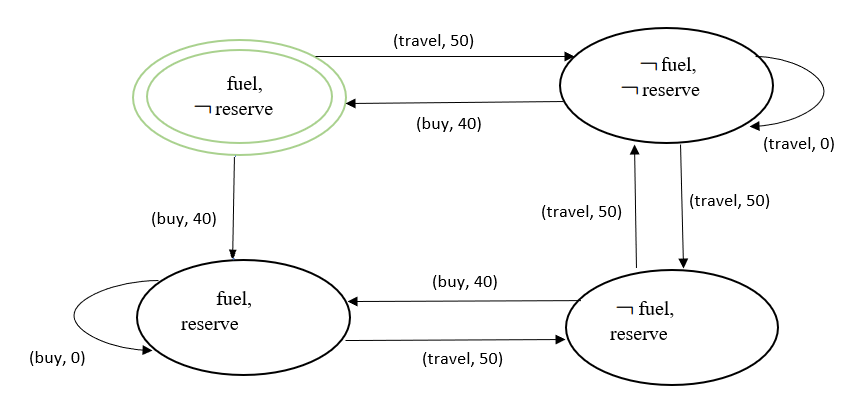
\includegraphics[width=6in,height=3in]{./media/ex01.png}
		\label{Figure:f01}
		\caption{Example 01}
	\end{figure}
	\subsection{Example 02}\label{example:ex02}
	\subsubsection{Description}\label{par:p102}
	John visits a painter to buy a specific painting. The cost of painting is 200\$ if its available in the shop. But if painting is not available then John needs to order a new one to be painted and will buy once its available.Order costs 50\$ At any time only one copy of painting is available and another one to be ordered once sold. 
	
	\subsubsection{Representation:}\label{par:p202}
	\indent 
	Fluents: available, sold.\\
	Actions: buy, order.\\
	Initially: ¬available, ¬sold\\
	buy causes sold if available\\
	buy causes ¬available\\
	buy costs 200$\$$ \\
	order causes available if ¬available\\
	order Cost: 50$\$$ \\
	order costs 50$\$$ \\
	
	\subsubsection{Calculation:}\label{par:p302}
	\indent \\
	$ \sum $ = $ \{ $ $ \sigma _{0}$, $ \sigma _{1}$, $ \sigma _{2}$, $ \sigma _{3}$$ \} $ \\
	$ \sigma _{0}$ = $ \{ $ ¬available, ¬sold$ \} $ \\
	$ \sigma _{1}$ = $ \{ $ available, ¬sold$ \} $ \\
	$ \sigma _{2}$ = $ \{ $ ¬available, sold$ \} $ \\
	$ \sigma _{3}$ = $ \{ $ available, sold$ \} $ \\
	\\
	\(  \Psi  \)  (buy, $ \sigma $0) = $ \sigma $0\\
	\(  \Psi  \)  (order, $ \sigma $0) = $ \sigma $1\\
	\(\Gamma\)(buy, $\sigma_{0}$) = 0\\
	\(\Gamma\)(order, $\sigma_{0}$) = 50\\
	\\
	\(  \Psi  \)  (buy $ \sigma $1) = $ \sigma $2\\
	\(  \Psi  \)  (order, $ \sigma $1) = $ \sigma $1\\
	\(\Gamma\)(buy, $\sigma_{1}$) = 200\\
	\(\Gamma\)(order, $\sigma_{1}$) = 0\\
	\\
	\(  \Psi  \)  (buy, $ \sigma $2) = $ \sigma $2\\
	\(  \Psi  \)  (order, $ \sigma $2) = $ \sigma $1\\
	\(\Gamma\)(buy, $\sigma_{2}$) = 0\\
	\(\Gamma\)(order, $\sigma_{2}$) = 50\\
	\\
	\(  \Psi  \)  (buy, $ \sigma $3) = $ \sigma $2\\
	\(  \Psi  \)  (order, $ \sigma $3) = $ \sigma $3\\
	\(\Gamma\)(buy, $\sigma_{3}$) = 200\\
	\(\Gamma\)(order, $\sigma_{3}$) = 0\\

	\subsubsection{Graph}\label{par:p402}
	\begin{figure}[H]
		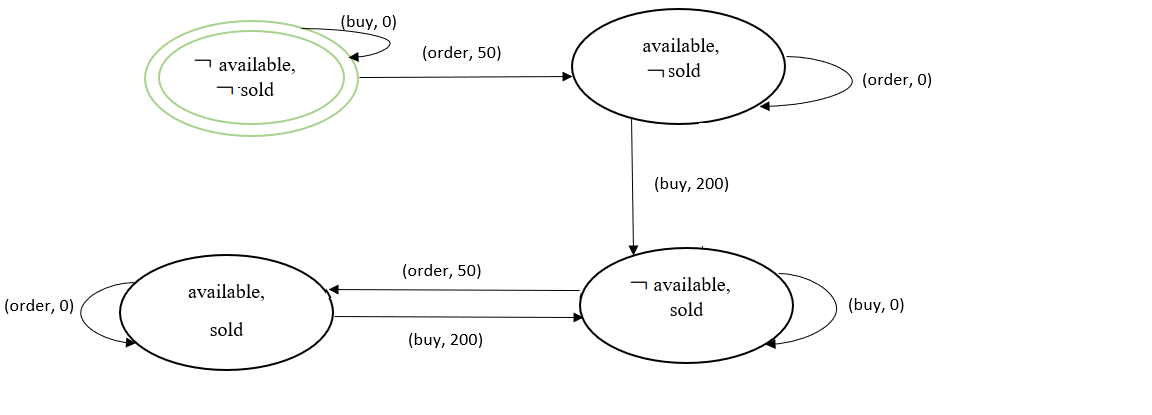
\includegraphics[width=1.2\linewidth, height=0.4\textheight]{./media/example2_graph.png}
		\label{Figure:f02}
		\caption{Example 02}
	\end{figure}
	\subsection{Example 03}
	\subsubsection{Description}\label{par:p103}
	There is a man. He can cook, eat, and play. Cooking makes food cooked. he can eat food if it is cooked. After eating he feels not hungry, and food is not cooked again. He can play. Playing makes him hungry. He just can play if he is not hungry. He just cooks when there is no food is cooked. Initially, he is hungry, and no food is cooked. In terms of energy, eating costs 5, cooking costs 15, playing costs 20.\\
	\\
	\subsubsection{Representation in language}\label{par:p203}
	Fluents: cooked, hungry.\\
	Actions: cook, eat, play.\\
	\\
	\\
	initially $\neg$cooked, hungry\\
	cook causes cooked if $\neg$cooked\\
	cook cost 15\\
	cook costs 15\\
	eat causes $\neg$cooked if cooked,hungry\\
	eat causes $\neg$hungry\\
	eat cost 5\\
	eat costs 5\\
	play causes hungry if $\neg$hungry\\
	play cost 20\\
	play costs 20\\
	\\
	\subsubsection{Calculation}\label{par:p303}
	$\sum$ = \{$\sigma_{0}$ ,$\sigma_{1}$, $\sigma_{2}$, $\sigma_{3}$\}\\
	\\
	$\sigma_{0}$ = \{$\neg$cooked, hungry\}\\
	$\sigma_{1}$ = \{cooked, hungry\}\\
	$\sigma_{2}$ = \{$\neg$cooked, $\neg$hungry\}\\
	$\sigma_{3}$ = \{cooked, $\neg$hungry\}\\
	\\
	\(  \Psi  \)(eat, $\sigma_{0}$) = $\sigma_{0}$\\
	\(  \Psi  \)(cook, $\sigma_{0}$) = $\sigma_{1}$\\
	\(  \Psi  \)(play, $\sigma_{0}$) = $\sigma_{0}$\\
	\(\Gamma\)(eat, $\sigma_{0}$) = 0\\
	\(\Gamma\)(cook, $\sigma_{0}$) = 15\\
	\(\Gamma\)(play, $\sigma_{0}$) = 0\\
	\\
	\(  \Psi  \)(eat, $\sigma_{1}$) = $\sigma_{2}$\\
	\(  \Psi  \)(cook, $\sigma_{1}$) = $\sigma_{1}$\\
	\(  \Psi  \)(play, $\sigma_{1}$) = $\sigma_{1}$\\
	\(\Gamma\)(eat, $\sigma_{1}$) = 5\\
	\(\Gamma\)(cook, $\sigma_{1}$) = 0\\
	\(\Gamma\)(play, $\sigma_{1}$) = 0\\
	\\
	\(  \Psi  \)(eat, $\sigma_{2}$) = $\sigma_{2}$\\
	\(  \Psi  \)(cook, $\sigma_{2}$) = $\sigma_{3}$\\
	\(  \Psi  \)(play, $\sigma_{2}$) = $\sigma_{1}$\\
	\(\Gamma\)(eat, $\sigma_{2}$) = 0\\
	\(\Gamma\)(cook, $\sigma_{2}$) = 15\\
	\(\Gamma\)(play, $\sigma_{2}$) = 20\\
	\\
	\(  \Psi  \)(eat, $\sigma_{3}$) = $\sigma_{2}$\\
	\(  \Psi  \)(cook, $\sigma_{3}$) = $\sigma_{3}$\\
	\(  \Psi  \)(play, $\sigma_{3}$) = $\sigma_{1}$\\
	\(\Gamma\)(eat, $\sigma_{3}$) = 5\\
	\(\Gamma\)(cook, $\sigma_{3}$) = 0\\
	\(\Gamma\)(play, $\sigma_{3}$) = 20\\
	\\
	\subsubsection{Graph}\label{par:p403}
	\begin{figure}[H]
		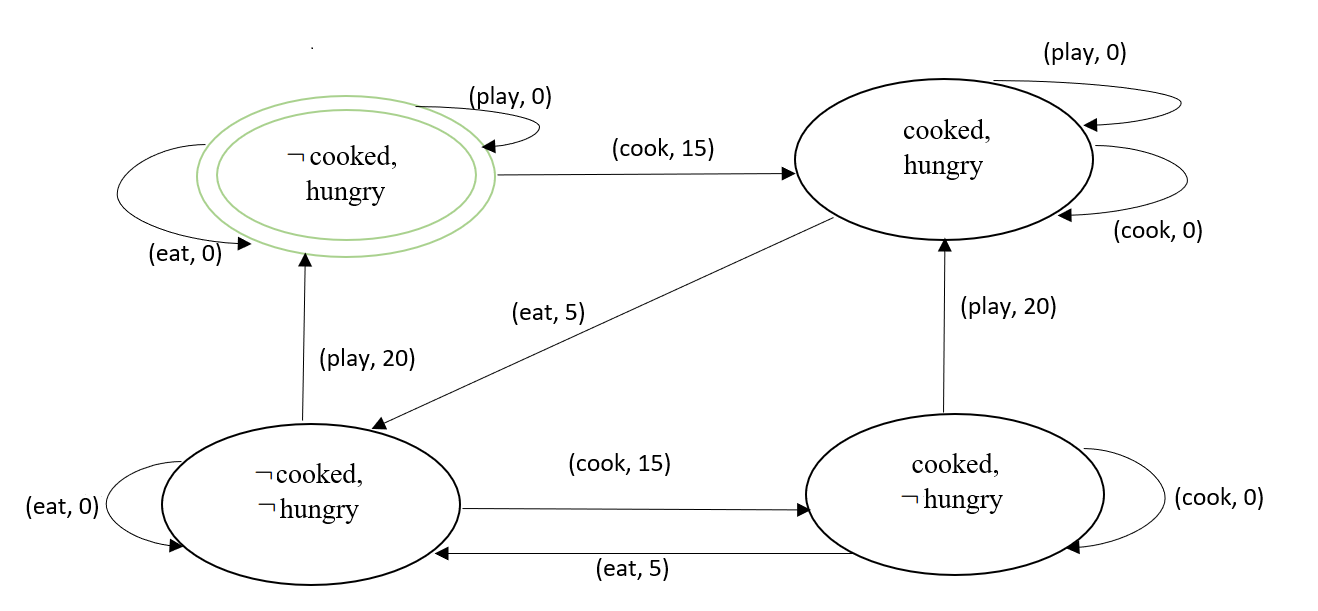
\includegraphics[width=1\linewidth, height=0.3\textheight]{./media/figure01.png}
		\caption{Example 03}
		\label{Figure:f03}
	\end{figure}
	\newpage
	\section{Appendix}	
	\begin{appendix}
		\listoffigures
		\listoftables
	\end{appendix}
\end{document}
